
% ----------------------------------------------------------------------
%  Set the document class
% ----------------------------------------------------------------------
\documentclass[11pt,a4paper,twoside]{article}

% ----------------------------------------------------------------------
% Define external packages, language, margins, fonts and new commands
% ----------------------------------------------------------------------
%\input{preamble} 
\usepackage[utf8]{inputenc}   % <<<<< Linux
\usepackage[english]{babel} % <<<<< English
\usepackage{notoccite}
\usepackage[skip=0.5\baselineskip]{caption}
\hyphenation{GTKWave}
\usepackage{listings}
\usepackage[all]{nowidow}
\usepackage{float}
%blind text
\usepackage{lipsum}
\usepackage{amsmath} 
\usepackage{graphicx}
\graphicspath{ {./} {../../figlib/}{../mat/}{../sim/} }
\def\FontLn{% 16 pt normal
  \usefont{T1}{phv}{m}{n}\fontsize{16pt}{16pt}\selectfont}
\def\FontLb{% 16 pt bold
  \usefont{T1}{phv}{b}{n}\fontsize{16pt}{16pt}\selectfont}
\def\FontMn{% 14 pt normal
  \usefont{T1}{phv}{m}{n}\fontsize{14pt}{14pt}\selectfont}
\def\FontMb{% 14 pt bold
  \usefont{T1}{phv}{b}{n}\fontsize{14pt}{14pt}\selectfont}
\def\FontSn{% 12 pt normal
  \usefont{T1}{phv}{m}{n}\fontsize{12pt}{12pt}\selectfont}

% Use Arial font as default
%
\renewcommand{\rmdefault}{phv}
\renewcommand{\sfdefault}{phv}
\usepackage{geometry}	
\geometry{verbose,tmargin=2.5cm,bmargin=2.5cm,lmargin=2.5cm,rmargin=2.5cm}

%\usepackage{setspace}
%\renewcommand{\baselinestretch}{1.5}

\usepackage[pdftex]{hyperref} % enhance documents that are to be
                              % output as HTML and PDF
\hypersetup{colorlinks,       % color text of links and anchors,
                              % eliminates borders around links
%            linkcolor=red,    % color for normal internal links
            linkcolor=black,  % color for normal internal links
            anchorcolor=black,% color for anchor text
%            citecolor=green,  % color for bibliographical citations
            citecolor=black,  % color for bibliographical citations
%            filecolor=magenta,% color for URLs which open local files
            filecolor=black,  % color for URLs which open local files
%            menucolor=red,    % color for Acrobat menu items
            menucolor=black,  % color for Acrobat menu items
%            pagecolor=red,    % color for links to other pages
            pagecolor=black,  % color for links to other pages
%            urlcolor=cyan,    % color for linked URLs
            urlcolor=black,   % color for linked URLs
	          bookmarks=true,         % create PDF bookmarks
	          bookmarksopen=false,    % don't expand bookmarks
	          bookmarksnumbered=true, % number bookmarks
	          pdftitle={report},
            pdfauthor={Andre C. Marta},
%            pdfsubject={Thesis Title},
%            pdfkeywords={Thesis Keywords},
            pdfstartview=FitV,
            pdfdisplaydoctitle=true}

\usepackage[numbers,sort&compress]{natbib} % <<<<< References in numbered list [1],[2],...
\usepackage{subcaption} 
\usepackage{mdframed}

%%%%%%%%%%%%%%%%%%%%%%%%%%%%%%%%%%%%%%%%%%%%%%%%%%%%%%%%%%%%%%%%%%%%%%%%
%     Begin Document                                                   %
%%%%%%%%%%%%%%%%%%%%%%%%%%%%%%%%%%%%%%%%%%%%%%%%%%%%%%%%%%%%%%%%%%%%%%%%


\begin{document}

% Set plain page style (no headers, footer with centered page number)
\pagestyle{plain}

% Set roman numbering (i,ii,...) before the start of chapters
%\pagenumbering{roman}

% ----------------------------------------------------------------------
%  Cover page
% ----------------------------------------------------------------------
%%%%%%%%%%%%%%%%%%%%%%%%%%%%%%%%%%%%%%%%%%%%%%%%%%%%%%%%%%%%%%%%%%%%%%%%
%                                                                      %
%     File: Thesis_FrontCover.tex                                      %
%     Tex Master: Thesis.tex                                           %
%                                                                      %
%     Author: Andre C. Marta                                           %
%     Last modified :  2 Jul 2015                                      %
%                                                                      %
%%%%%%%%%%%%%%%%%%%%%%%%%%%%%%%%%%%%%%%%%%%%%%%%%%%%%%%%%%%%%%%%%%%%%%%%

\thispagestyle {empty}

% IST Logo - Signature A
% parameters: bb=llx lly urx ury (bounding box), width=h_length, height=v_length, angle=angle, scale=factor, clip=true/false, draft=true/false. 
\includegraphics[bb=9.5cm 11cm 0cm 0cm,scale=0.29]{IST_A_CMYK_POS}

\begin{center}
%
% Figure (Image or plot)
\vspace{1.0cm}
% height = 50 mm
%\includegraphics[height=50mm]{Figures/Airbus_A350.jpg}

% Title, author and degree
\vspace{1cm}
{\FontLb Circuit Theory and Electronics Fundamentals} \\ % 
\vspace{1cm}
{\FontSn Engineering Physics} \\ % <<<<< EDIT COURSE
\vspace{1cm}
{\FontSn Lab 5: Bandpass filter using OPAMP} \\
\vspace{1cm}
{\FontSn Beatriz Rosalino (96514), Mariana Ribeiro (96552), Sofia Guerreiro (96567)} \\
\vspace{1cm}
{\FontSn 6 June, 2021} \\ % <<<<< EDIT DATE (corresponds to date of oral examination)
%
\end{center}



% ----------------------------------------------------------------------
% Dedication page (optional)
% ----------------------------------------------------------------------
%\input{dedication} 
%\cleardoublepage

% ----------------------------------------------------------------------
%  Acknowledgments (optional)
% ----------------------------------------------------------------------
%\input{acknowledgements}
%\cleardoublepage

% ----------------------------------------------------------------------
%  Abstract (both in English and Portuguese)
% ----------------------------------------------------------------------
%\input{resumo} 
%\cleardoublepage

%\input{abstract} 

% ----------------------------------------------------------------------
%  Table of contents, list of tables, list of figures and nomenclature
% ----------------------------------------------------------------------

% Table of contents
%
\tableofcontents

% List of tables
%\addcontentsline{toc}{section}{\listtablename}
%\listoftables
%\cleardoublepage 

% List of figures
%\addcontentsline{toc}{section}{\listfigurename}
%\listoffigures
%\cleardoublepage 

% Set arabic numbering (1,2,...) after preface
%
%\setcounter{page}{1}
%\pagenumbering{arabic}

% ----------------------------------------------------------------------
%  Body
% ----------------------------------------------------------------------

\section{Introduction}
\label{sec:intro}
The main goal of this work is to analyze an RC circuit and study its various responses to a voltage source that changes over time. First, we studied the behavior of the circuit when the voltage imposed on the capacitor was constant and non zero (Section ~\ref{ssec:tl}), then we studied the natural response of the capacitor (voltage source imposing voltage equal to 0) in (Section ~\ref{ssec:n}), the forced response (voltage source imposing sinusoidal voltage) in (Section ~\ref{ssec:fs}), over time. We also studied the circuit for different frequencies of the sinusoidal signal, plotting the voltages at the capacitor and the nodes of its terminals as functions of frequency Section ~\ref{ssec:freq}.\\

Our circuit (Figure ~\ref{fig:circuit}) consists of 7 resistors, 2 voltage sources - 1 independent, and 1 current controlled dependent one, 1 independent current source and 1 capacitor.\\
The voltage provided by the independent source follows the equation:
\begin{equation}\label{eqn:vss}
\begin{split}
{v_s (t)} = \left\{\begin{array}{ll} \ V_s ,  \quad \ \  if \ \  \ t \leq 0 \\ 
 \ sin(2 \pi f t) , \quad \ \  if \ \ \ t \textgreater 0 \end{array} \right.
  \end{split}
\end{equation}
\begin{figure}[H] \centering
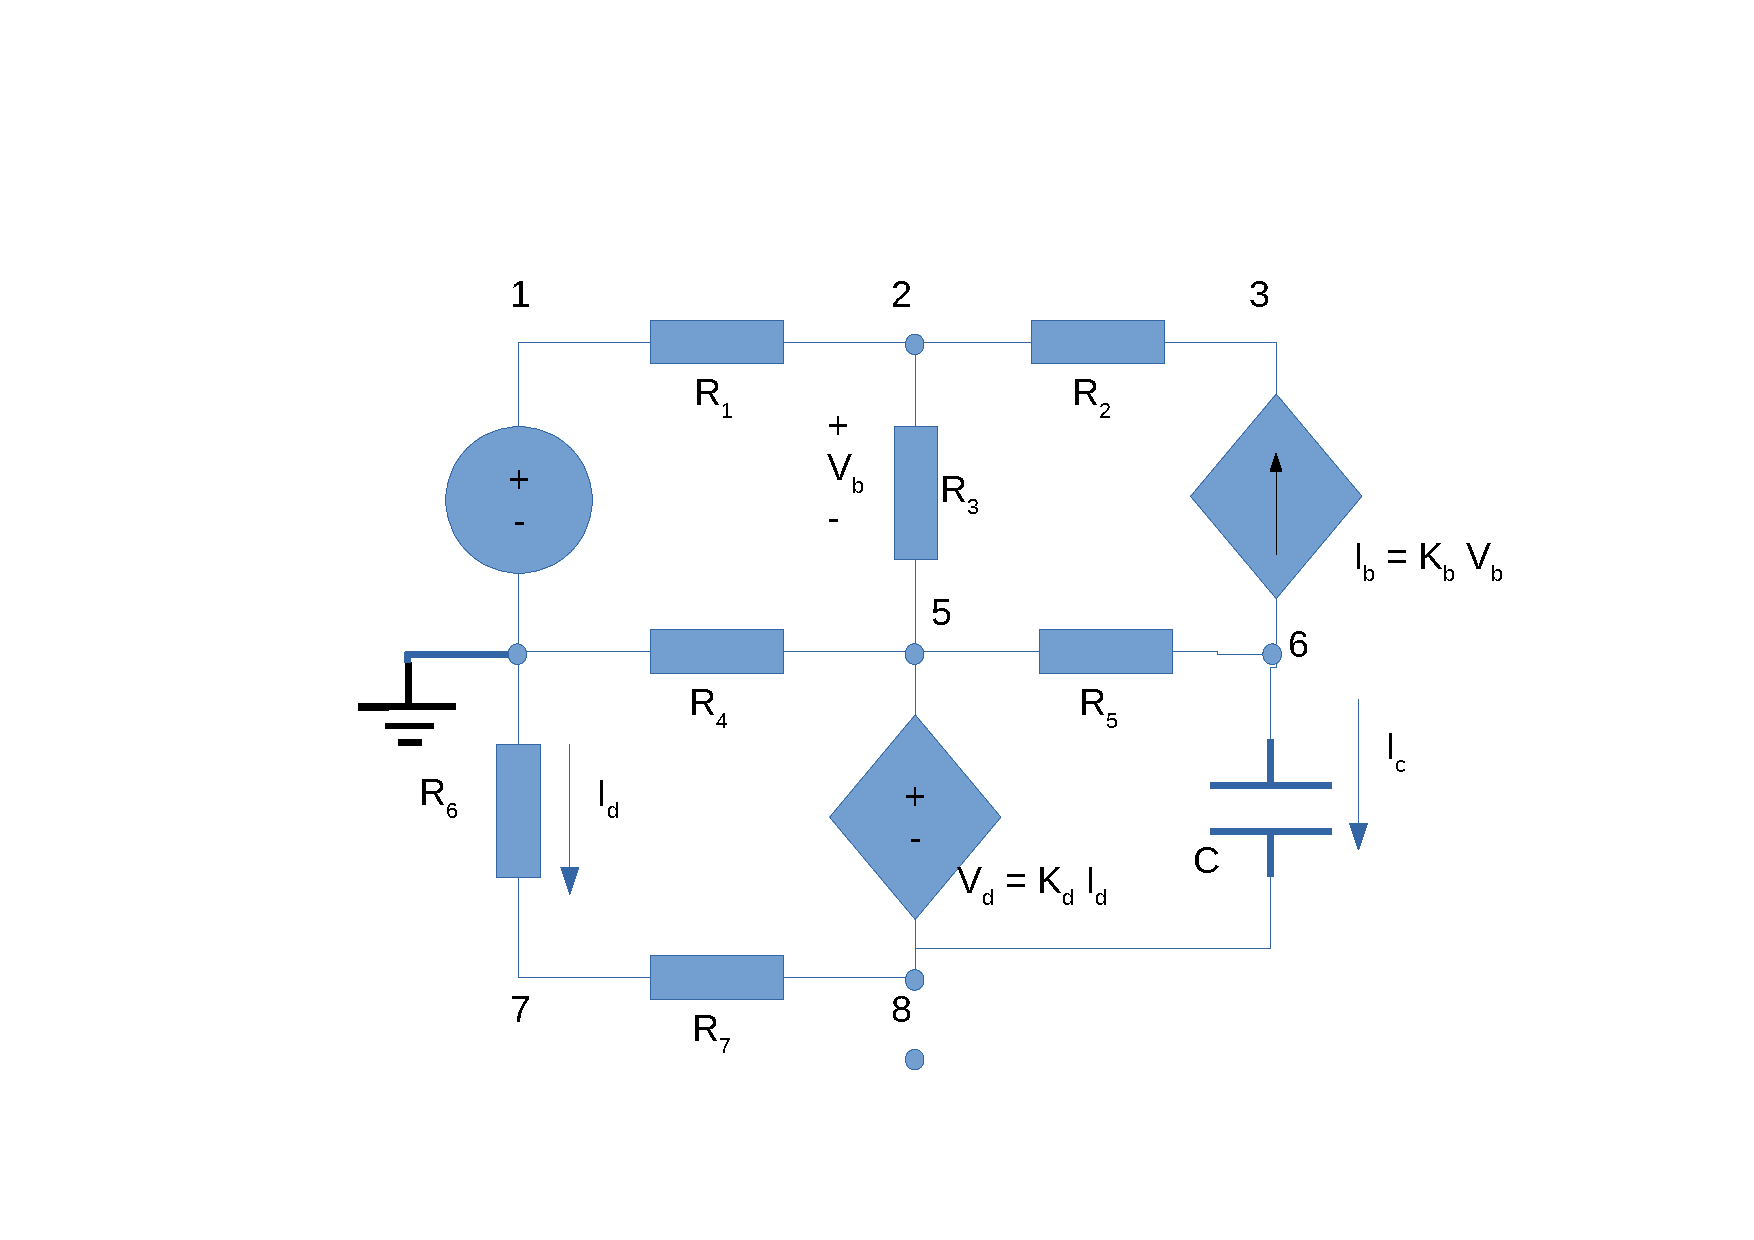
\includegraphics[width=0.8\linewidth]{circuito.pdf}
\caption{Circuit}
\label{fig:circuit}
\end{figure} 
We wrote a system of equations for each theoretical analysis, from Kirchhoff and Ohm's Laws. To get the solutions and plots for these analysis, we used \textit{octave}, which solved our systems of equations efficiently and gave us all currents and voltages for all branches. We then used \textit{ngspice} to get a simulation of this circuit, expecting to obtain the same results. We compared the results from different methods in the conclusion (Section ~\ref{sec:conclusion}).


\section{Theoretical analysis}
\label{sec:ta}
\subsection{Operating point analysis for t\textless0}
\label{ssec:tl}
For t\textless0, from equation (por aqui equação da função de ramos da voltagem) we can see that $v_s (t)= V_s$. That means the voltage source drives constant voltage $V_s$. We consider that enough time has passed for the capacitor to fully charge from this constant voltage, so the voltage at nodes 6 and 8 are the same and there is no current flowing through the capacitor (it now acts as an open circuit). Removing the part of the circuit that is an open circuit we get a "new" circuit, that is easy to analyse: \\
\begin{figure}[H] \centering
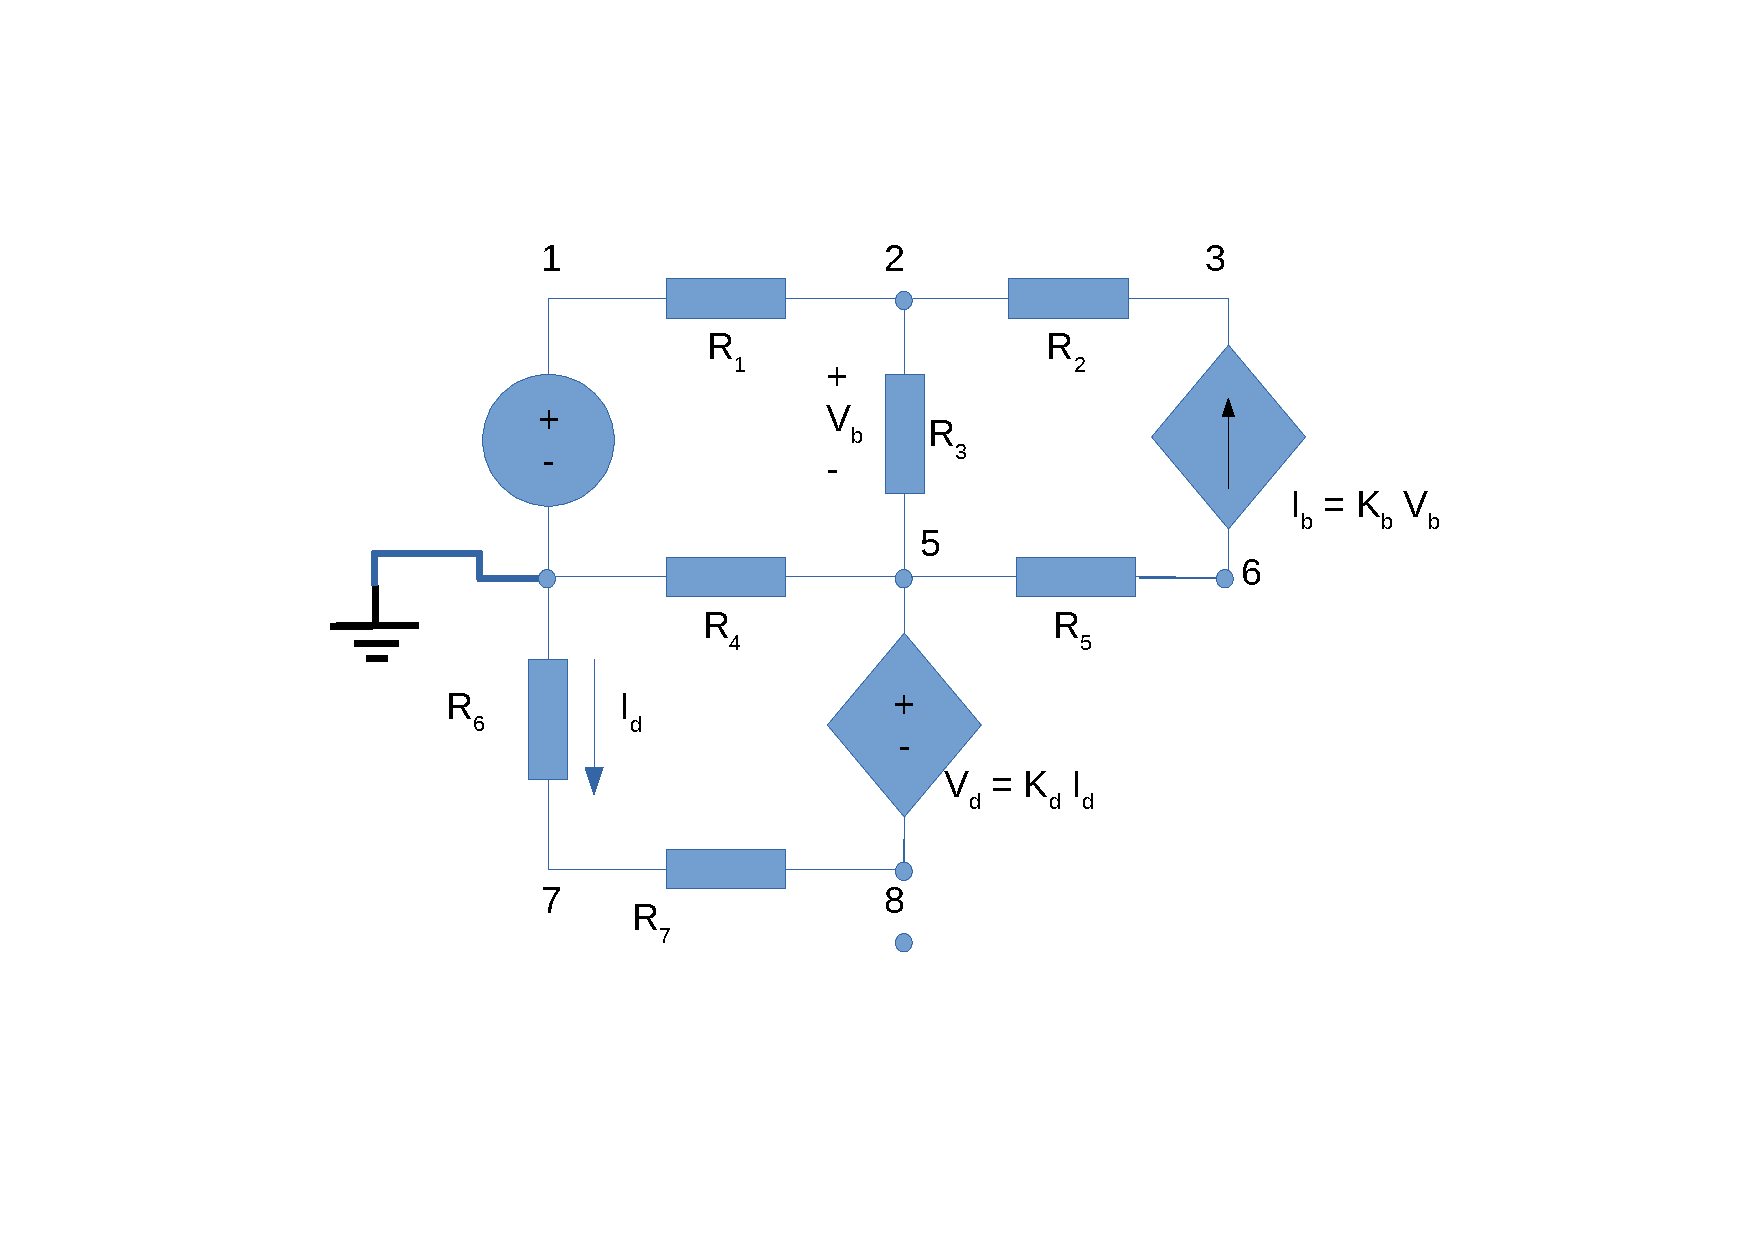
\includegraphics[width=0.8\linewidth]{tmenor0.pdf}
\caption{Circuit to analyse for t\textless0}
\label{fig:zim}
\end{figure}

In this circuit, there are 8 nodes, one of which is a ground node (the one that connects $R_4$, the voltage source and $R_6$. Therefore, to solve the circuit we must find 7 independent equations. \\
To discover the equations for each node we need to use Kirchhoff’s Current Law, which states that the sum of all the currents entering and leaving a node must be equal to zero. For simplicity instead of using directly the currents we will also use Ohm's Law and we will consider that all currents are leaving the nodes. \\
The equations for the 7 nodes are:
\begin{equation}
    V_{1}=V_{s} 
\end{equation}
\begin{equation}
  \frac{V_{2}-V_{1}}{R_{1}} +\frac{V_{2}-V_{3}}{R_{2}}+\frac{V_{2}-V_{5}}{R_{3}}=0 
\end{equation}
\begin{equation}
  V_{5}-V_{2}+\frac{V_{3}-V_{2}}{R_{2} K_b}=0
\end{equation}
\begin{equation}
   \frac{V_{5}}{R_{4}} + \frac{V_{5}-V_{6}}{R_{5}}+ \frac{V_{8}-V_{7}}{R_{7}} + \frac{V_{5}-V_{2}}{R_{3}}=0 
\end{equation}
\begin{equation}
    \frac{V_{3}- V_{2}}{R_{2}} + \frac{V_{6}-V_{5}}{R_{5}} = 0
\end{equation}
\begin{equation}
    V_{7}+ R_6 \left(\frac{V_{7}-V_{8}}{R_{7}}\right) = 0
\end{equation}
\begin{equation}
  V_{8}-V_{5} + K_d \left(\frac{V_{8}-V_{7}}{R_{7}}\right) = 0
\end{equation}
\\
The next step is to solve the system of equations: \\
\\
\begin{equation}
\left(\begin{array}{ccccccc} 
1 & 0 & 0 & 0 & 0 & 0 & 0\\
-\frac{1}{R_1} & \frac{1}{R_1}+\frac{1}{R_2}+\frac{1}{R_3} & -\frac{1}{R_2} & -\frac{1}{R_3}& 0 & 0 & 0 \\
0 & -1-\frac{1}{R_2 K_b} & \frac{1}{R_2 K_b} & 1 & 0 & 0 & 0 \\
0 & -\frac{1}{R_3} & 0 & \frac{1}{R_3} +\frac{1}{R_4}+\frac{1}{R_5} & -\frac{1}{R_5} & -\frac{1}{R_7} & \frac{1}{R_7} \\
0 & -\frac{1}{R_2} & \frac{1}{R_2} & -\frac{1}{R_5} & \frac{1}{R_5} & 0 & 0 \\
0 & 0 & 0 & 0 & 0 & 1+\frac{R_6}{R_7} & -\frac{R_6}{R_7} \\
0 & 0 & 0 & -1 & 0 & -\frac{K_d}{R_7} & 1 + \frac{K_d}{R_7} \\
\end{array}\right)
\left(\begin{array}{c} V_1 \\ V_2 \\ V_3 \\ V_5 \\ V_6 \\ V_7 \\ V_8 \end{array}\right) 
= \left(\begin{array}{c} V_s\\ 0 \\ 0 \\ 0 \\0 \\ 0 \\0 \end{array}\right)
\end{equation}

\subsection{Determination of Equivalent Resistor($R_{eq}$)}
\label{ssec:R}
Just as suggested, we made $V_s = 0$ and replaced the capacitor with a voltage source $V_x= V(6)-V(8)$, where V(6) and V(8) are the voltages in nodes 6 and 8 as obtained in section ~\ref{ssec:tl}. Then, we did once again the nodal analysis, with the purpose of obtaining values for $I_x$ and $V_x$, since we need this to get $R_{eq}$ for further analysis. To get this resistance, on the capacitor terminals, we need to use Thévenin's theorem. We are considering the capacitor, so, to get Thévenin's equivalent, we need to have an open circuit at the capacitor terminals. The rest of the circuit will be a voltage source $V_{Th}$ in series with a resistor of $R_{eq}=R_{Th}$ so the voltage drop across $R_{eq}$ is  $V_{Th}-0= V_{Th}$. In this way,  $V_{Th}$ will be equal to the open-circuit voltage, which is the voltage at the capacitor terminals. So to get Thévnin's equivalent circuit, we susbtitute the capacitor with a voltage source of voltage $V_{Th}$. This voltage source will have to have voltage $V_x$ to guartee the necessary continuity of voltage in the capacitor, from t\textless0.\\
\begin{figure}[H] \centering
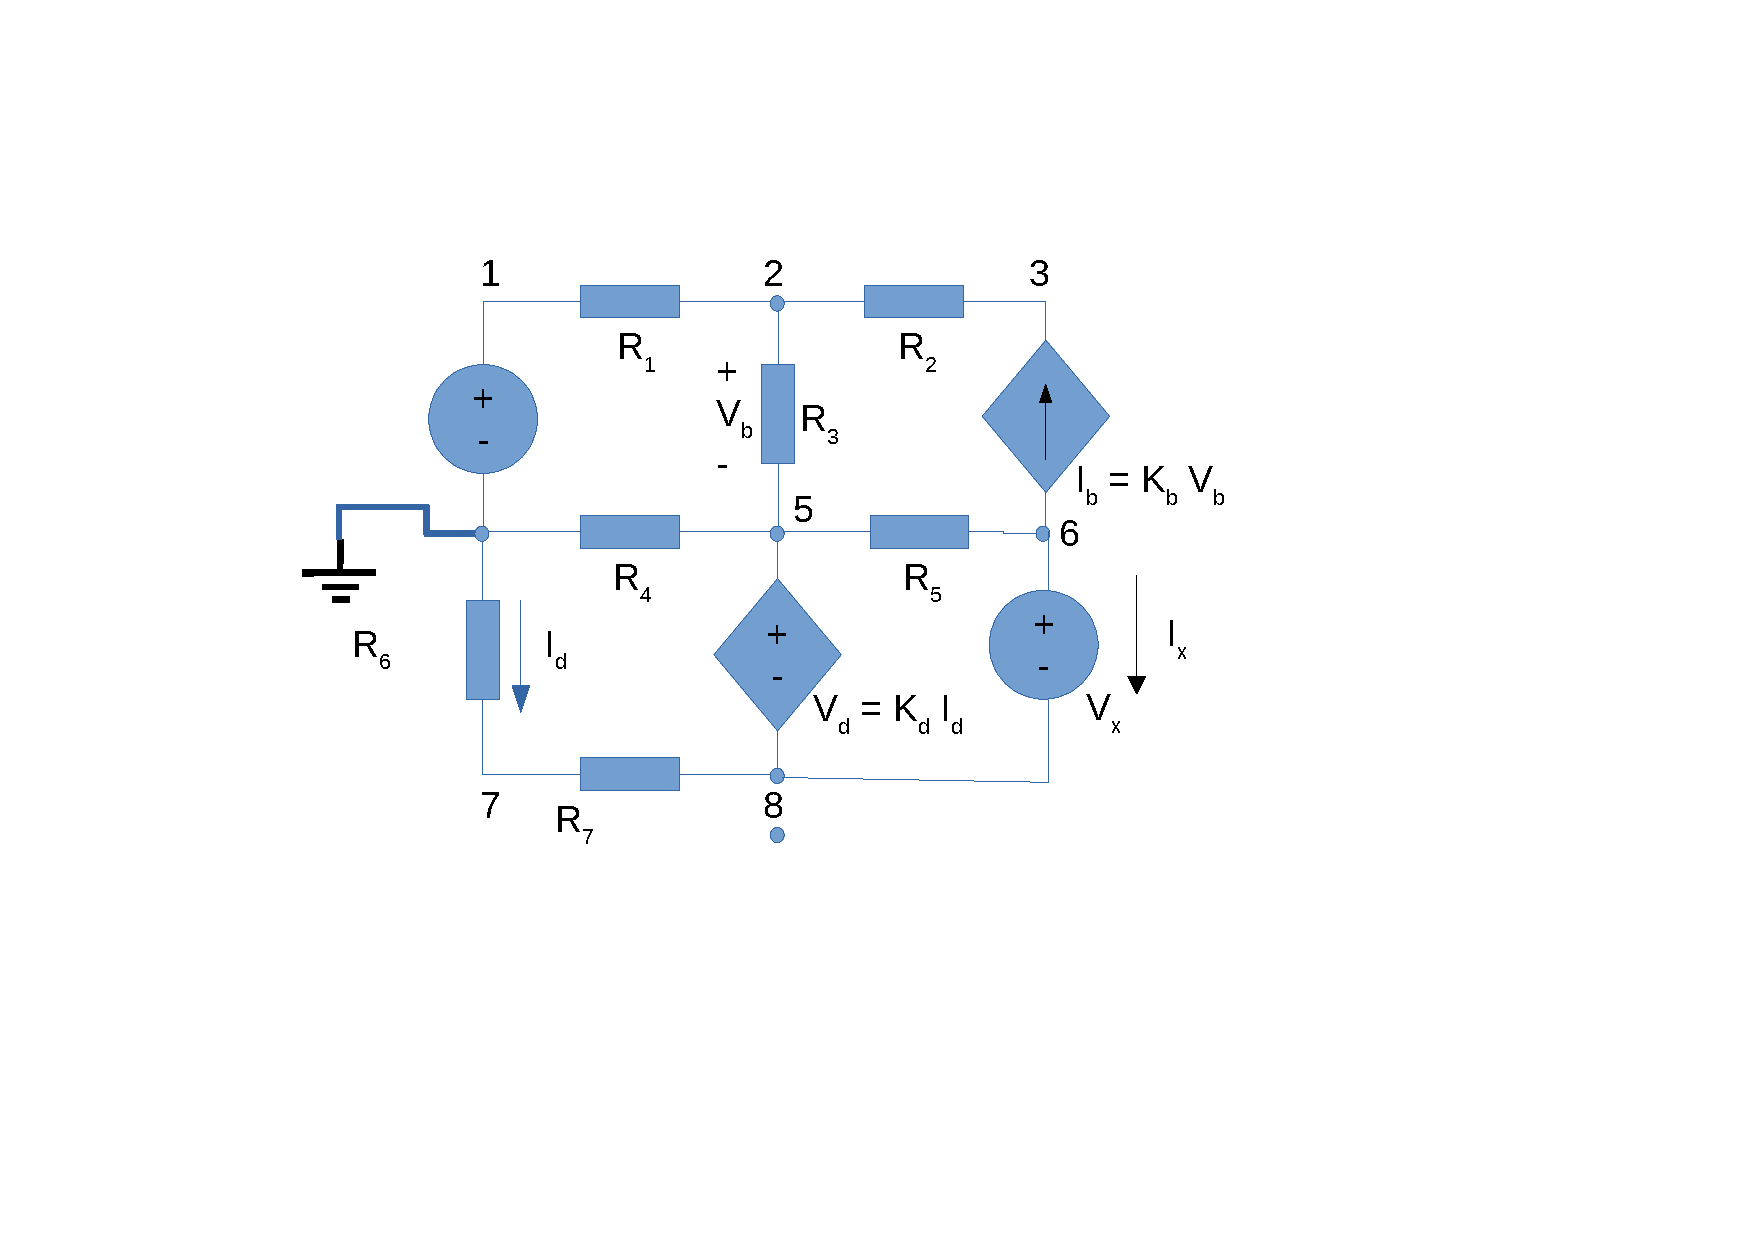
\includegraphics[width=0.8\linewidth]{vx.pdf}
\caption{Circuit for t=0}
\label{fig:zim}
\end{figure}
Now, we only need 6 equations, because the GND node and node 1 become the same node.\\
For node 2, we get:
\begin{equation}
\frac{V_2}{R_1} + \frac{V_2 - V_3}{R_2} + \frac{V_2 - V_5}{R_3} = 0 \Leftrightarrow V_2\left( \frac{1}{R_1} + \frac{1}{R_2} + \frac{1}{R_3} \right) - \frac{V_3}{R_2} - \frac{V_5}{R_3}=0
\end{equation}

For node 3:
\begin{equation}
\frac{V_3 - V_2}{R_2\times K_b }+ V_5 - V_2 = 0 \Leftrightarrow V_2 \left(-\frac{1}{R_2\times K_b} - 1\right) + \frac{V_3}{R_2\times K_b} + V_5 = 0
\end{equation}

For node 5, we get:
\begin{equation} \label{eqn:n5}
  \frac{V_5}{R_4}+ \frac{V_5-V_2}{R_3} + \frac{V_5-V_6}{R_5} + i_d= 0
\end{equation}

Where $i_d$ is the current passing trough the dependent voltage source, $V_d$, ($i_d = -(I_d + I_x)$).

For node 6, we get:
\begin{equation} \label{eqn:n6}
  I_b + \frac{V_6-V_5}{R_5} + I_x = 0 \Leftrightarrow I_x = \frac{V_2-V_3}{R_2} + \frac{V_5-V_6}{R_5}
\end{equation}

And also:
\begin{equation}
V_6-V_8 = V_x
\end{equation}

For node 7:
\begin{equation}
-I_d + \frac{V_7-V_8}{R_7} = 0 \Leftrightarrow \frac{V_7}{R_6} - \frac{V_7-V_8}{R_7} = 0\Leftrightarrow V_7\left(\frac{1}{R_6} + \frac{1}{R_7}\right) - \frac{V_8}{R_7} = 0
\end{equation}

Combining equations (\eqref{eqn:n5}), (\eqref{eqn:n6}) and noticing that $I_d = \frac{V_7-V_8}{R_7}$:
\begin{equation}
V_2 \left( -\frac{1}{R_2} - \frac{1}{R_3}\right) + \frac{V_3}{R_2} +  V_5 \left( \frac{1}{R_3} + \frac{1}{R_4}\right) - \frac{V_7}{R_7} + \frac{V_8}{R_7} = 0
\end{equation}

Knowing that $I_d = \frac{V_d}{K_d}$ and $I_d = \frac{V_7-V_8}{R_7}$, we get the final equation:
\begin{equation}
V_8\left( \frac{1}{R_7} - \frac{1}{K_d}\right) - \frac{V_7}{R_7} + \frac{V_5}{K_d}
\end{equation}


The next step is to solve the following system of equations:
\begin{equation}
\left(\begin{array}{cccccc} \frac{1}{R_1}+\frac{1}{R_2} +\frac{1}{R_3} & -\frac{1}{R_2} & -\frac{1}{R_3} & 0 & 0 & 0\\ -\frac{1}{R_2 K_b}-1 & \frac{1}{R_2 K_b} & 1 & 0 & 0 & 0 \\ -\frac{1}{R_2}-\frac{1}{R_3} & \frac{1}{R_2} & \frac{1}{R_3}+\frac{1}{R_4} & 0& -\frac{1}{R_7} &\frac{1}{R_7} \\ 0&0&0&1&0&-1\\0&0&0&0&\frac{1}{R_6}+\frac{1}{R_7}&-\frac{1}{R_7} \\ 0&0&\frac{1}{K_d}&0&-\frac{1}{R_7}&\frac{1}{R_7}-\frac{1}{K_d}\end{array}\right)
\left(\begin{array}{c} V_2 \\ V_3 \\ V_5 \\ V_6 \\ V_7 \\ V_8 \end{array}\right) 
= \left(\begin{array}{c} 0 \\ 0 \\ 0 \\ V_x \\ 0 \\ 0 \end{array}\right)
\end{equation}

Finally, we can calculate $I_x$ using equation \eqref{eqn:n6}, the equivalent resistance $R_{eq}$ and the time constant, $\tau$: 
\begin{equation}
R_{eq}=\frac{V_x}{I_x}
\end{equation}
\begin{equation}
\tau=R_{eq}\times C
\end{equation}

\subsection{Natural Solution}
\label{ssec:n}
The natural solution only depends on initial charge (voltage) and on the time constant. The voltage source $V_s$ needs to be turned off to get the natural response of the system, so $V_s=0$ and  $V_{6n}(t)$ becomes
\begin{equation}
  V_{6n}(t) = Ae^{-\frac{t}{\tau}}
\end{equation}
With the results obtained in section ~\ref{ssec:R}, we get both $A=V_{6n}(0)=V_x$,and the time constant $\tau$. We will plot the results in the time interval [0, 20] ms. \\


\subsection{Forced solution}
For t>0, the voltage source has the form $v_s(t)=sin(2 \pi  f t)$, where $f$ represents the frequency of the sinusoidal excitation. We expect that if we allow the system to evolve for a sufficient amount of time (enough that the natural solution dies out), the voltage at node 6 (the node near the capacitor) will also tend towards a sinusoidal signal. \\
Since this circuit has a lot of components, it helps to use phasor notation, in which the voltages become the real part of complex vectors (called phasors), with information about the magnitude and phase of the signal. When we do nodal analysis we can ignore the time dependance and introduce it at the end, multiplying the phasors by the term $e^{2 \pi f t j}$, where $f$ is the forced frequency (imposed by the voltage source), taking finally the real combination of sine and cosine functions. \\
Since we are using phasors, where voltages and currents are complex numbers, we also need to substitute the capacitor with its impedance (which is the resistance equivalent for phasors). The impedance of the capacitor can be expressed by $z_{c}=\frac{1}{2 \pi f C j}$. \\
The new nodal equations become: \\
\begin{equation}
    V_{1}=V_{s}=1
\end{equation}
\begin{equation}
  \frac{V_{2}-V_{1}}{R_{1}} +\frac{V_{2}-V_{3}}{R_{2}}+\frac{V_{2}-V_{5}}{R_{3}}=0 
\end{equation}
\begin{equation}
  V_{5}-V_{2}+\frac{V_{3}-V_{2}}{R_{2} K_b}=0
\end{equation}
\begin{equation}
   \frac{V_{5}}{R_{4}} + \frac{V_{5}-V_{6}}{R_{5}}+ \frac{V_{8}-V_{7}}{z_c} + \frac{V_{5}-V_{2}}{R_{3}}=0 
\end{equation}
\begin{equation}
    \frac{V_{3}- V_{2}}{R_{2}} + \frac{V_{6}-V_{5}}{R_{5}} + \frac{V_{6}-V_{8}}{z_c} = 0
\end{equation}
\begin{equation}
    V_{7}+ R_6 \left(\frac{V_{7}-V_{8}}{R_{7}}\right) = 0
\end{equation}
\begin{equation}
  V_{8}-V_{5} + K_d \left(\frac{V_{8}-V_{7}}{R_{7}}\right) = 0
\end{equation}
The system of equations in matrix form: \\
\left(\begin{array}{ccccccc} 
1 & 0 & 0 & 0 & 0 & 0 & 0\\
-\frac{1}{R_1} & \frac{1}{R_1}+\frac{1}{R_2}+\frac{1}{R_3} & -\frac{1}{R_2} & -\frac{1}{R_3}& 0 & 0 & 0 \\
0 & -1-\frac{1}{R_2 K_b} & \frac{1}{R_2 K_b} & 1 & 0 & 0 & 0 \\
0 & -\frac{1}{R_3} & 0 & \frac{1}{R_3} +\frac{1}{R_4}+\frac{1}{R_5} & -\frac{1}{R_5} & -\frac{1}{z_c} & \frac{1}{z_c} \\
0 & -\frac{1}{R_2} & \frac{1}{R_2} & -\frac{1}{R_5} & \frac{1}{R_5} + \frac{1}{z_c} & 0 & -\frac{1}{z_c}\\
0 & 0 & 0 & 0 & 0 & 1+\frac{R_6}{R_7} & -\frac{R_6}{R_7} \\
0 & 0 & 0 & -1 & 0 & -\frac{K_d}{R_7} & 1 + \frac{K_d}{R_7} \\
\end{array}\right)
\left(\begin{array}{c} V_1 \\ V_2 \\ V_3 \\ V_5 \\ V_6 \\ V_7 \\ V_8 \end{array}\right) 
= \left(\begin{array}{c} 1 \\ 0 \\ 0 \\ 0 \\0 \\ 0 \\0 \end{array}\right)

\subsection{Final Solution}
The final solution for $V_6(t)$ incorporates the natural and forced solution:
\begin{equation}
V_6(t) = V_{6n}(t) + V_{6f}(t)
\end{equation}
Before $V_6(t)$ is a constant (and so is $V_s(t)$), but in the instant t = 0, $V_6(0)=V_x$ and $V_s(0) = 0$. Then, for t > 0, $V_s(t) = sin(2\pi ft)$ and $V_6(t)$, from de sections ~\ref{section:n} and ~\ref{}, is:
\begin{equation}
V_6(t) = R(V_6)\times sin(wt)+Im(V_6)\times cos(wt)+Aexp(-\frac{t}{\tau})
\end{equation}
Finally, using \textit{Octave}, we plotted both $V_s(t)$ and $V_6(t)$ in the same figure in the interval [-5, 20] ms.
\subsection{Frequency response}
A transfer function is a function that computes output from input. In the case of an RC circuit such as the one being studied here, the transfer function is simply the quotient of phasors, the phasor correspondent to the voltage of the capacitor ($v_c (t)$) and the phasor correspondent to the voltage source ($v_s (t)$):
\[ T(\omega)= \frac{\widetilde{v_c}}{\widetilde{v_s}}=\frac{1}{1+j\omega R C}\]
Since the transfer function is complex, we can represent its magnitude and phase as functions of $\omega$. 
\[ |T(\omega)|= \frac{1}{\sqrt{1+\omega^2 R^2 C^2}}\]

\section{Simulation}
\label{sec:simulation}
In this circuit, we have a current dependent voltage source between nodes 5 and 8, so that, to sense the controlling current, $I_d$, between nodes GND and 7, we need to use a voltage source of voltage 0V, to sense said current. For this purpose, we placed this source between node 7 and a new node - node 9-, which connects the negative terminal of the voltage source and resistor 7, so that it is in series with resistor 6, through which $I_d$ flows, and therefore senses that same current.\\
\subsection{Operating Point Analysis for t\textless0}
To simulate the response of the circuit for t\textless0, where the voltage source introduces to the circuit a constant voltage, $V_s$, the current through the capacitor is zero, so there is an open circuit between nodes 6 and 8. The results of the operating point analysis for this circuit, t\textless0, obtained using \textit{ngspice}, can be seen in Table (ref).\\

\subsection{Operating Point Analysis for t=0}
To get the operating point analysis for t=0, knowing $v_s(0)=0$, we substitute the capacitor, between nodes 6 and 8, with a voltage source $V_x=V_6-V_8$, where $V_6$ and $V_8$ are the voltage for nodes 6 and 8, respectively, obtained in the previous op analysis (for t\textless0). This is needed so continuity of voltage in the capacitor is guaranteed. The results of this analysis, using \testit{ngspice} can be seen in Table (ref).\\
\subsection{Transient Analysis for Natural Response}
From now on, we have a capacitor in its place, between nodes 6 and 8.\\
To simulate the natural response of the circuit, the source $V_s$ was turned off(the voltage has to be 0V to get the natural response), and we used boundary conditions of $V_6$ and $V_8$(voltages in nodes 6 and 8), as the values obtained in t=0. These conditions will also be used in the latter sections. We did transient analysis, for the [0,20]ms time interval, with a 0.02ms time step. The plot of $v_{6}(t)$ is shown in Figure(ref).\\
\subsection{Analysis of Total Response}
For this section, we now have $V_s$ as a sine wave of frequency f=1k Hz, and amplitude 1 ($V_s=sin(2\pi f t)$). A transient analysis was done, for nodes 6 (V6) and 1 (Vs),again for the [0,20]ms time period with a 0.02ms time step. We can then see the results of the voltage introduced to the circuit (Vs) and the total response on node 6, from both this stimulus from Vs and the natural response of the system. This can be seen in Figure (ref).\\
\subsection{Frequency Analysis}
To evaluate the circuit when the frequency changes, we used ac analysis, by decades - using a frequency logscale. Frequencies were considered from 0.1 Hz to 1MHz and we used 100 points to plot both the magnitude and phase of voltages of nodes 1, 6 and of the capacitor $v_c$, which corresponds to $V_6 - V_8$, as functions of frequency. The magnitude plot can be seen in Figure (ref), and the phase plot in Figure (ref).\\

\section{Results}
\label{sec: res}

\subsection{Plots}
The results obtained from the analysis in Section ~\ref{sec: sim} can be seen in Figure ~\ref{fig:rc1}.
\begin{figure}[H] \centering
  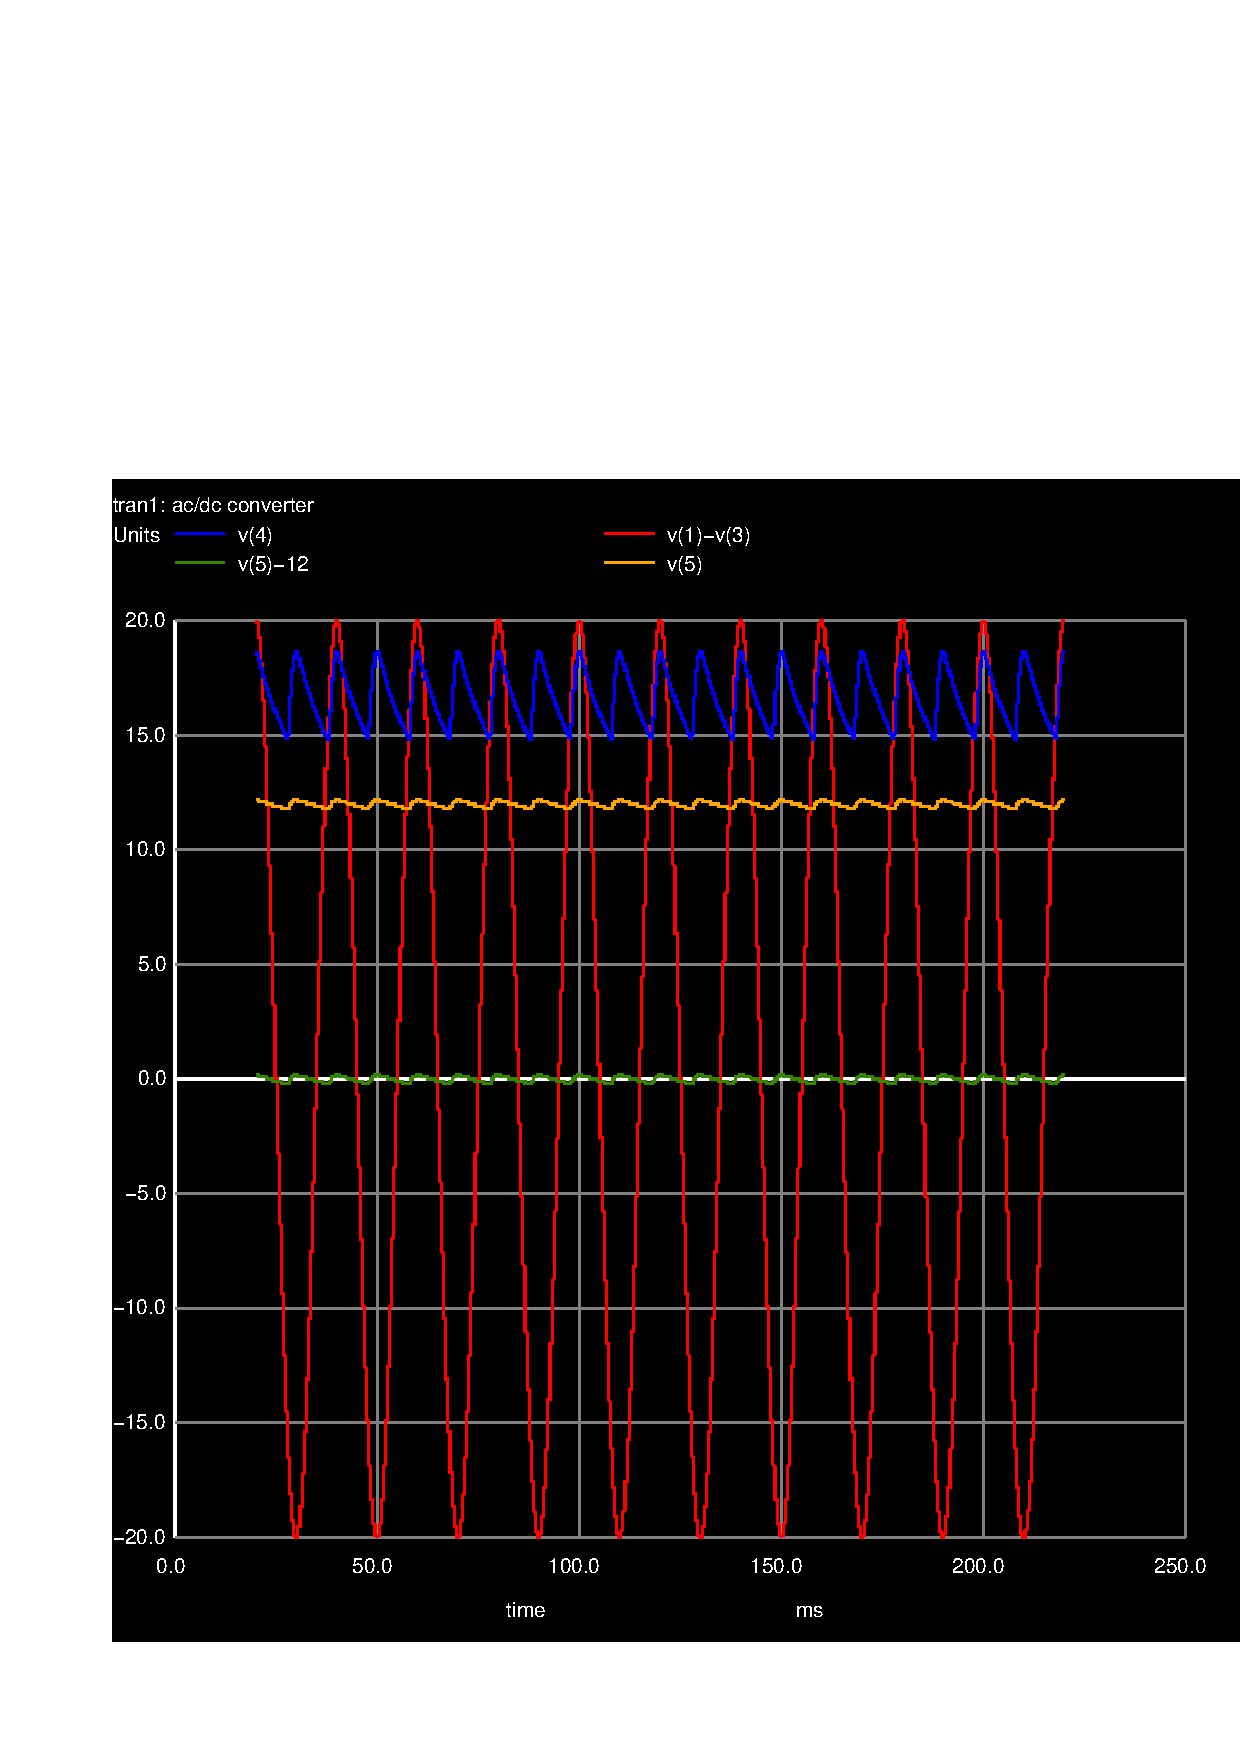
\includegraphics[width=0.6\linewidth]{vospice50.pdf}
\caption{Voltage simulation plots over time: red - voltage in secondary winding; blue - envelope detector output voltage; yellow - voltage regulator output voltage; green - ripple}
\label{fig:rc1}
\end{figure}

From Section ~\ref{sec:theo} we obtained one period of the waves, seen in Figures ~\ref{fig:vo} to ~\ref{fig:vofinal}. 

\begin{figure}[H] \centering
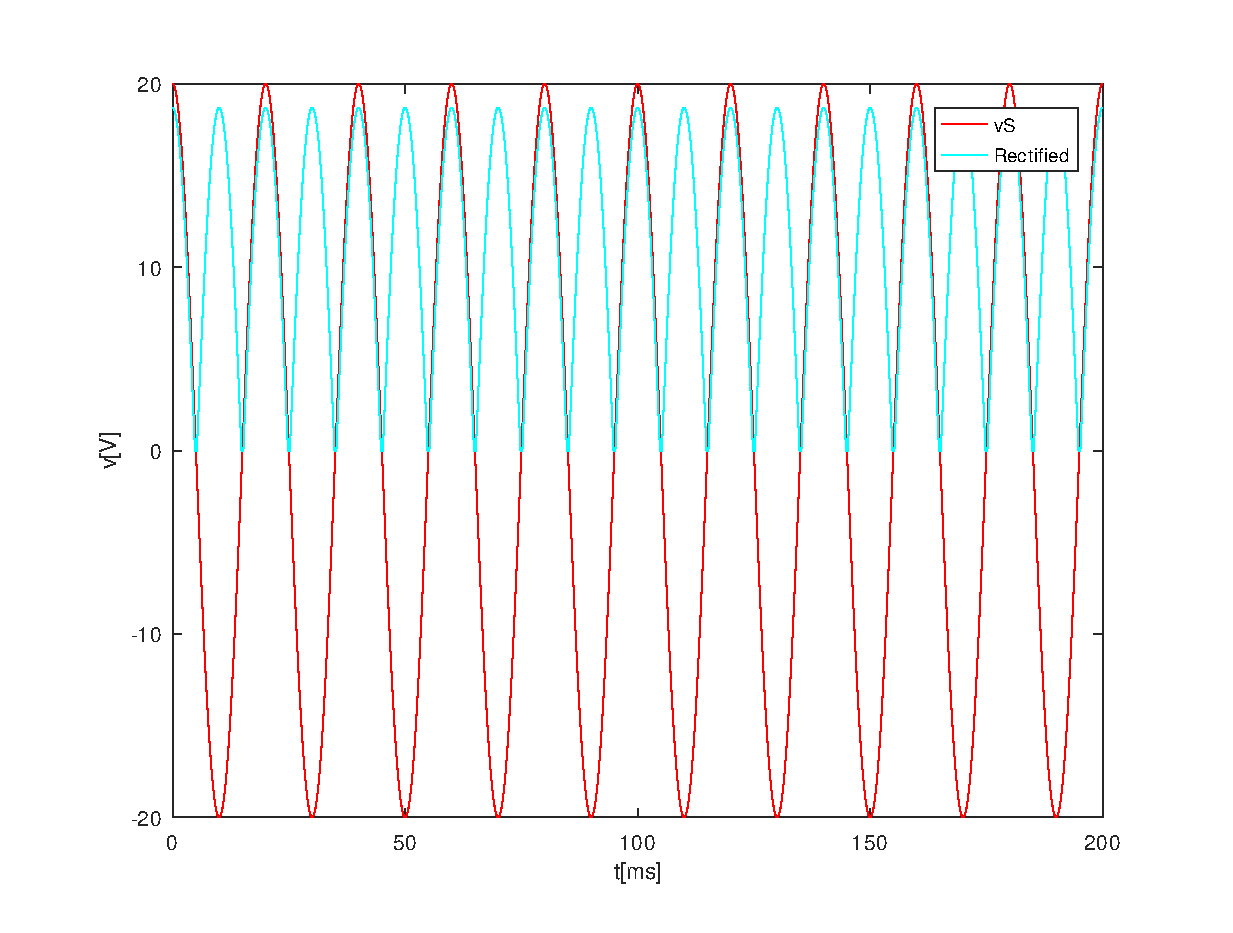
\includegraphics[width=0.4\linewidth]{vo.eps}
\caption{Voltage in the secondary winding (red) and voltage in rectifier (cyan) over time}
\label{fig:vo}
\end{figure}

\begin{figure}[H] \centering
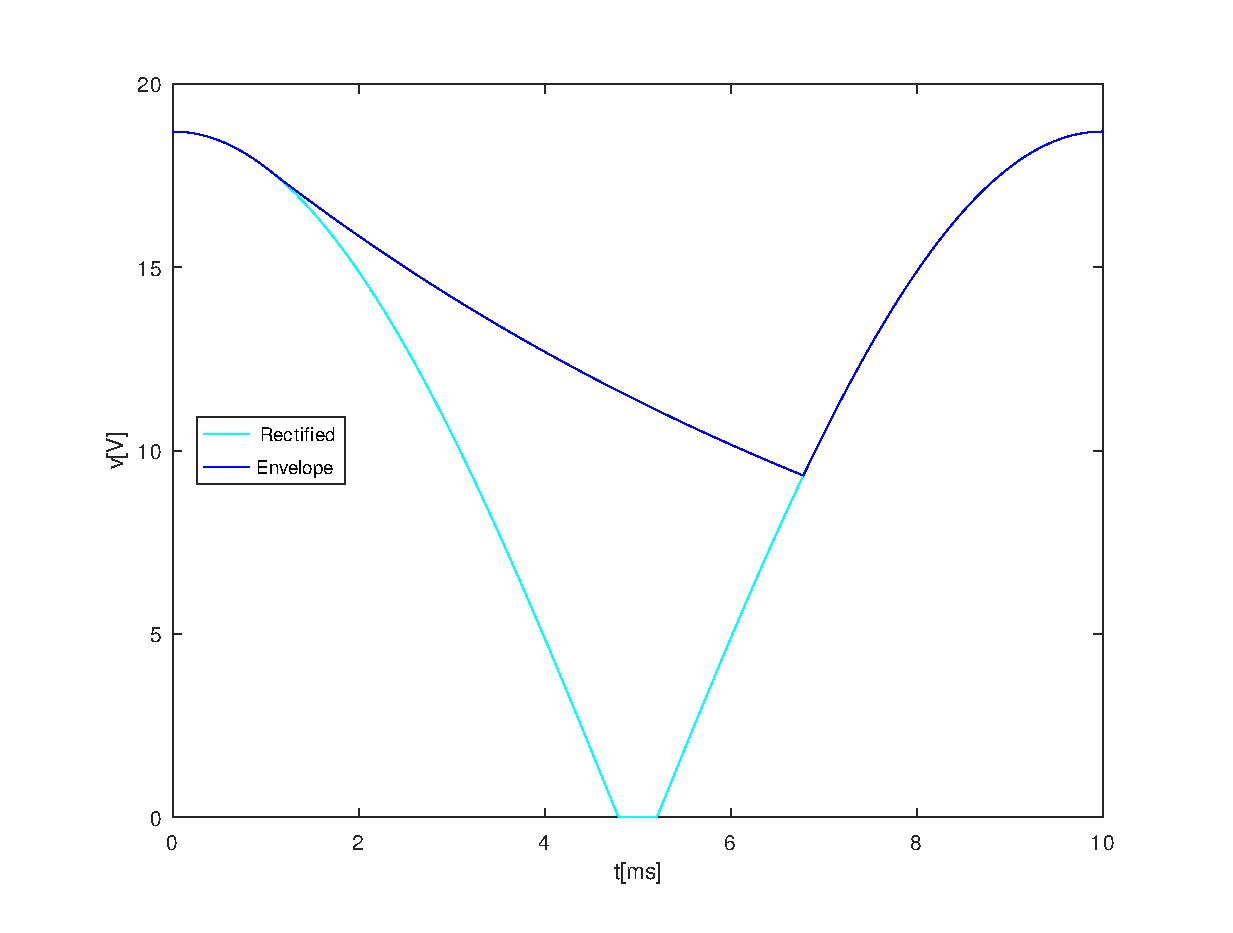
\includegraphics[width=0.4\linewidth]{venvlope.eps}
\caption{Envelope detector output voltage (blue) and voltage in rectifier (cyan) over one period}
\label{fig:voen}
\end{figure}

\begin{figure}[H] \centering
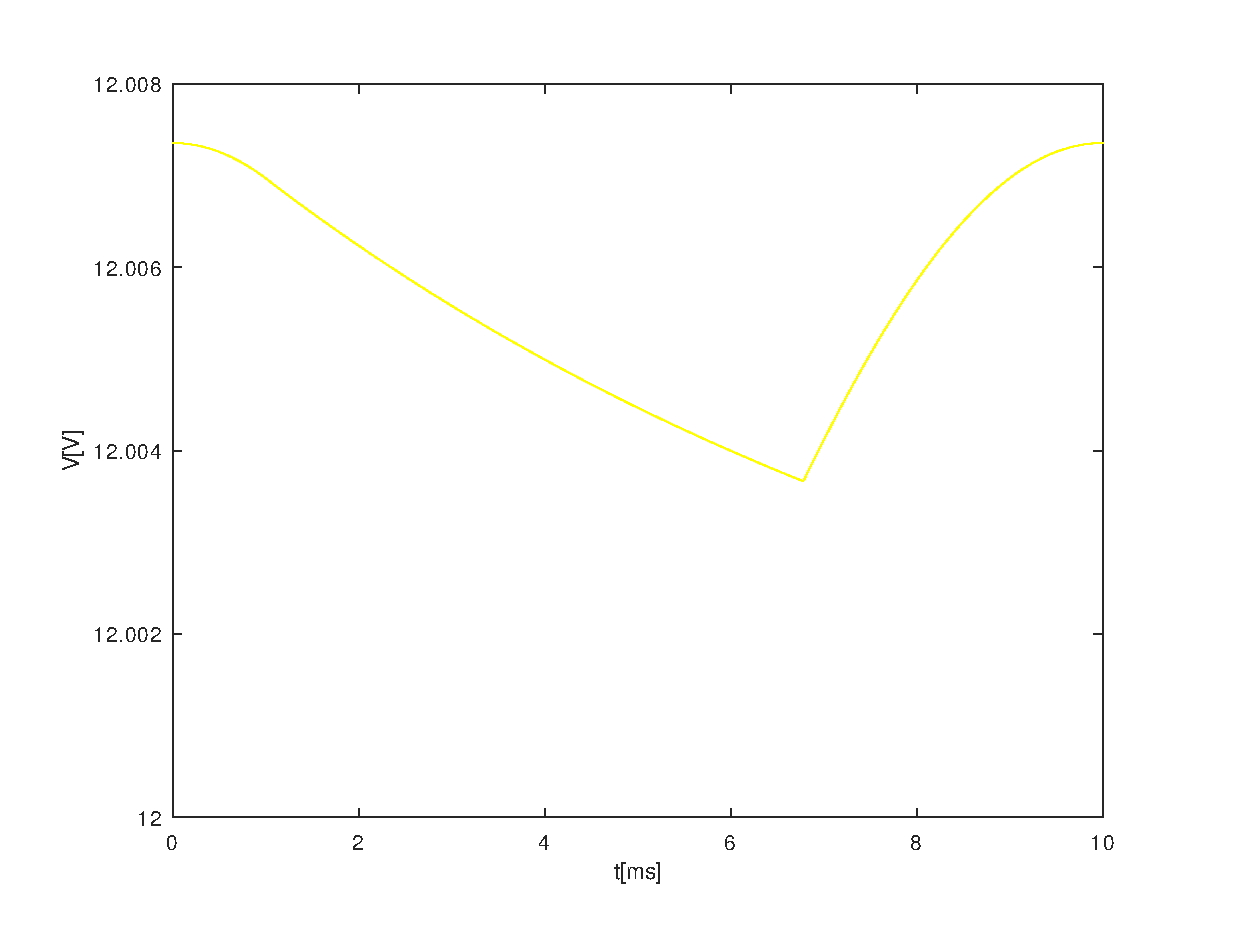
\includegraphics[width=0.4\linewidth]{vregulator.eps}
\caption{Voltage regulator output voltage over one period}
\label{fig:voreg}
\end{figure}

\begin{figure}[H] \centering
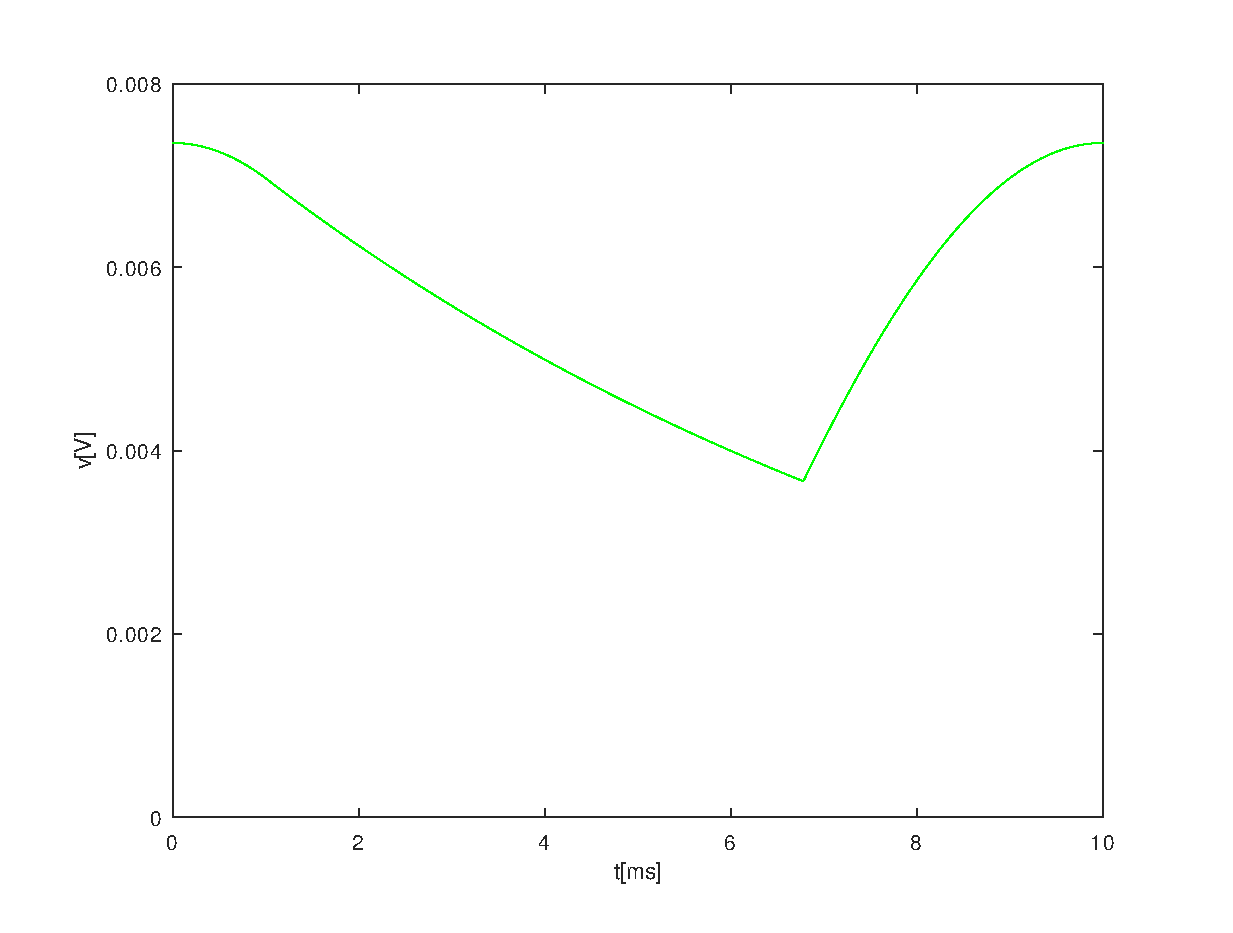
\includegraphics[width=0.4\linewidth]{vfinal.eps}
\caption{Ripple over one period}
\label{fig:vofinal}
\end{figure}

\subsection{Merit}
To calculate the merit we used the following equation:
\begin{equation}
M = \frac{1}{cost(ripple(v_O) + average(v_O - 12) + 10^{-6})}
\end{equation}
The cost is the sum of the cost of the resistor (1 MU/k$\Omega$), the capacitor (1 MU/$\mu$F) and the diodes (0.1 MU/diode). Our total cost is 8.2 MU.\\
The DC output level average was calculated using function average() in \textit{ngspice} and function mean() in \textit{octave}. The results were 11.99012V and 12.007V, respectively.\\
The ripple was calculated using functions max() and min() in both \textit{ngspice} and \textit{octave}. The results were 0.35752V and 0.00036995V, respectively.\\
The merit was only calculated for the \textit{ngspice} simulation and the result was 0.3319.

\section{Conclusion}
\label{sec:conclusion}
In this laboratory assignment, the objective of analysing the RC circuit has been achieved. \\
When looking at the tables of currents and voltages obtained by \textit{Octave} and \textit{ngspice} for the analysis of the circuit when t\textless 0 we can that they perfectly match, which is expected since all components considered are linear.\\
In the analysis for t=0, just one voltage is different than 0, $V_6$, and both methods resulted in the same value for this voltage, and for the current that goes throught $R_5$. In the \textit{ngspice} simulation the rest of voltages, that were supposed to be zero (and were, in the table obtained by \textit{Octave}), are in fact values of very small order of magnitude being practically negligible, which checks out.\\
In terms of all of the plots, the ones obtained by \textit{Octave} were a perfect match for the ones obtained in \textit{ngspice}.\\
Only the magnitude plot regarding $V_6$ had differences, when comparing both tools, since they seem to be mirrored.

%\cleardoublepage

% ----------------------------------------------------------------------
%  Bibliography
% ----------------------------------------------------------------------
%\addcontentsline{toc}{section}{\bibname}
%\bibliographystyle{abbrvunsrtnat} % <<<<< SELECT IF USING REFERENCES BY NUMBER (CITATION ORDER)
%\bibliography{../../../BIBfile.bib}

% ----------------------------------------------------------------------
\end{document}
% ----------------------------------------------------------------------

